\documentclass[tikz,border=0pt]{standalone}
\usepackage{pgfplots}
\usepackage{xcolor}

\begin{document}
\begin{tikzpicture}
  [
    rec0/.style={shade,
                rectangle,
                minimum width=4mm,
                minimum height=1.5mm,
                inner sep=0pt,
                outer sep=0pt,
                top color=gray!60!white,
                bottom color=gray!30!white,
                draw=black, 
                very thin},
    rec16/.style={shade,
                rectangle,
                rotate=16,
                minimum width=4mm,
                minimum height=1.5mm,
                inner sep=0pt,
                outer sep=0pt,
                top color=gray!60!white,
                bottom color=gray!30!white,
                draw=black, 
                very thin},
    rec16r/.style={shade,
                rectangle,
                rotate=-16,
                minimum width=4mm,
                minimum height=1.5mm,
                inner sep=0pt,
                outer sep=0pt,
                top color=gray!60!white,
                bottom color=gray!30!white,
                draw=black, 
                very thin},
    rec45/.style={shade,
                rectangle,
                rotate=45,
                minimum width=20mm,
                minimum height=7.5mm,
                inner sep=0pt,
                outer sep=0pt,
                top color=gray!60!white,
                bottom color=gray!30!white,
                draw=black, 
                very thin}
  ]
\begin{scope}
    \node[inner sep=0pt]  at (0,0)
        {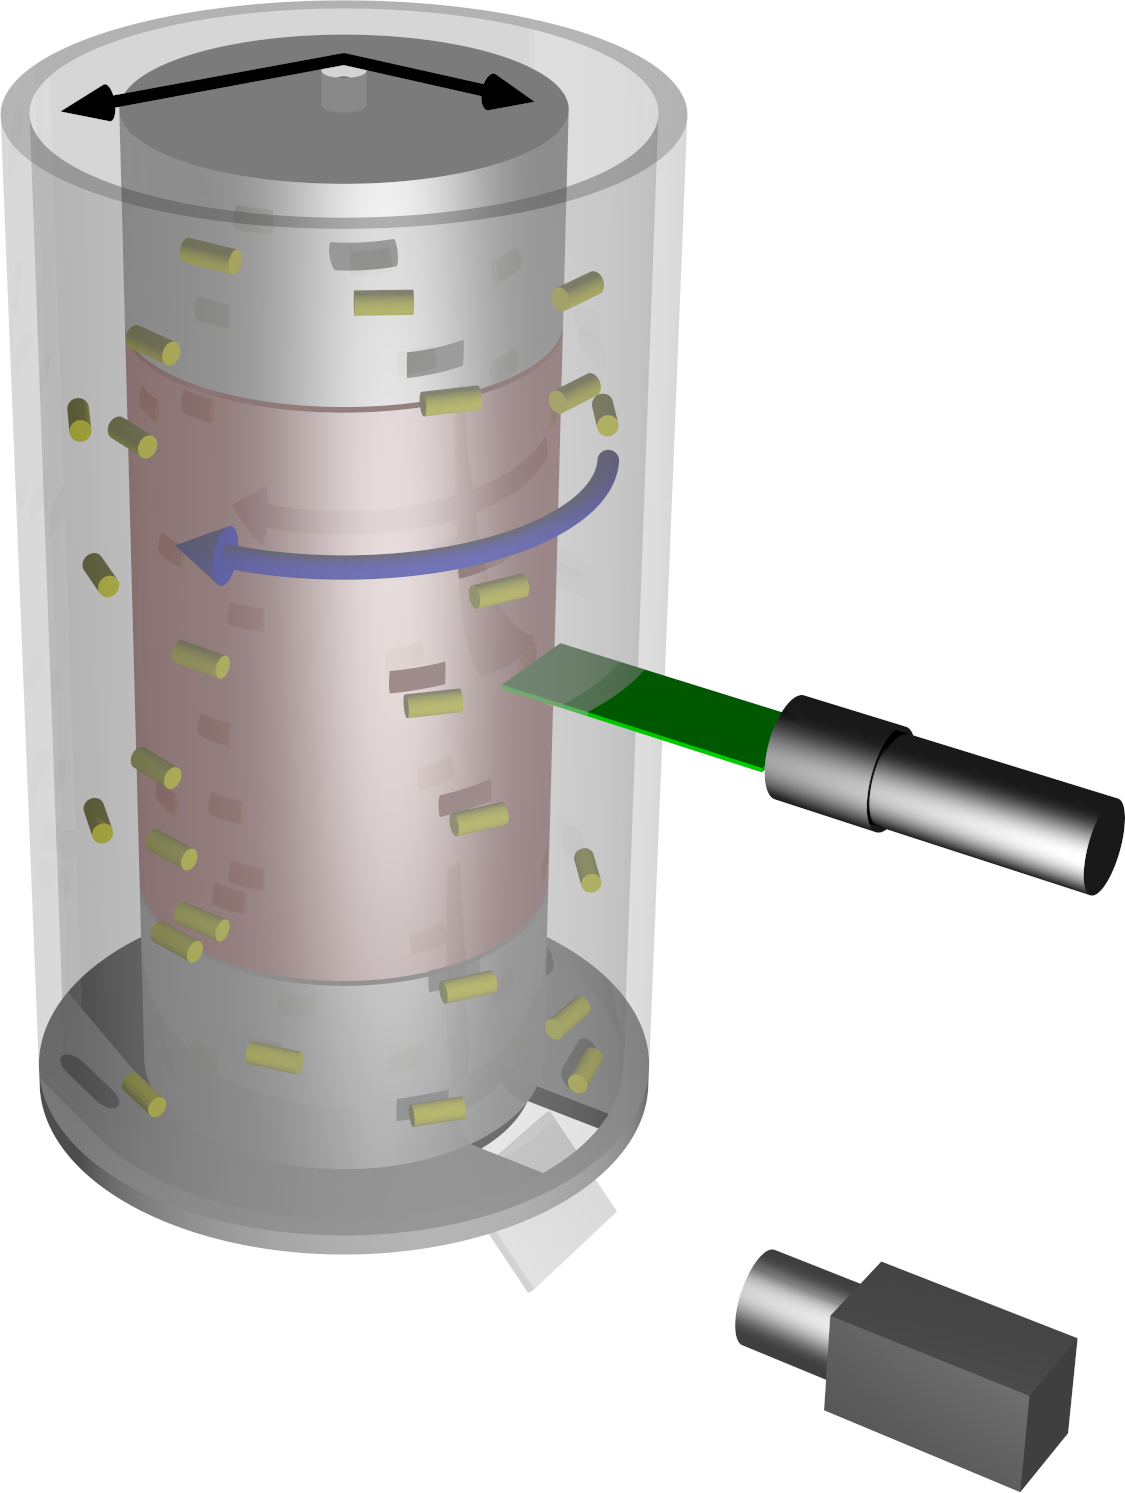
\includegraphics[height=7cm]{t3csetup.png}};
\end{scope}


\begin{scope}[
    xshift=6.cm,
    yshift=4.0cm
    ]

    \begin{scope}[
         scale=4,
         every node/.append style={transform shape},
        ]
        \clip (-0.487, -1.220) rectangle (0.502, -1.86);
    
        % Outer cylinder and water inside
        \draw[color=black, fill=white, thin] (0, 0) circle (1.851);
    
        % inner cylinder
        \draw[color=black, fill=gray!10, thin] (0, 0) circle (1.325);
    
        \draw[color=black, dashed, thick] (-0.487, -1.25) -- (-0.487, -1.79);
        \draw[color=black, dashed, thick] (0.502, -1.243) -- (0.502, -1.79);
        \draw[color=black, dashed, thick] (-0.487, -1.220) -- (0.502, -1.220);
        \node at (0.025, -1.275) {\scalebox{0.28}{IC}};
    
        % dashed center line
        \draw[color=red, thick, densely dotted] (0, 0) circle (1.588);

        % filled polygon
        \coordinate (L1) at (-0.487, -1.79);
        \coordinate (L2) at (-0.487, -1.233);
        \coordinate (L3) at (-0.360, -1.275);
        \fill[color=red, opacity=0.2] (L1) -- (L2) -- (L3) -- cycle;
        \coordinate (R1) at (0.502, -1.79);
        \coordinate (R2) at (0.502, -1.228);
        \coordinate (R3) at (0.375, -1.272);
        \fill[color=red, opacity=0.2] (R1) -- (R2) -- (R3) -- cycle;
    
     \end{scope}
    
        % plot fiberes
        \path (0, -6.352) coordinate[rec0];  
        \path (-1.70, -6.12) coordinate[rec16r];  
        \path (1.75, -6.10) coordinate[rec16];  
    
    % big fiber representation
    \begin{scope}[
         yshift=15mm,
         xshift=5mm
        ]
        \path (0, -3.50) coordinate[rec45];  
        \draw[color=black, densely dashed, thick] (-1.5, -5) -- (1.10, -2.4);
        \draw[color=red, thick] (-2, -3.5) -- (1.10, -3.5);
        \draw[color=blue] (-1.5, -3.5) arc (180:225:15mm);
        \node at (-1.70, -4.25) {\scalebox{1.5}{$\theta_p$}};
        
    \end{scope}
\end{scope}
    
    % labels
    \node at (-3.0, 3.25) {(a)};
    \node at (3.65, 3.25) {(b)};
    \node at (3.65, -0.50) {(c)};

    \node at (-0.9, 1.3) {\huge$-\omega_i$};
    \node at (-0.6, 3.4) {\huge$r_i$};
    \node at (-1.7, 3.4) {\huge$r_o$};

\end{tikzpicture}
\end{document}
